\documentclass[fontset=windows, 12pt]{article}
\usepackage{Article}
\usepackage{lshort-zh-cn-style}
\usepackage{layout}
\usepackage{booktabs}
\newcommand{\Cmd}[2][\{*args\}]{\texttt{\textbackslash#2#1}}

%% 1. 书籍章节符号
\usepackage[object=vectorian]{pgfornament}
\usepackage{lipsum,tikz}
\usepackage{tcolorbox}
% \usepackage{emoji}
\newcommand{\Test}[2][default *args]{第一个参数:\texttt{#1}\\第二个参数:#2}
\tcbuselibrary{theorems}
\tcbset{highlight math/.append style={left=0mm,right=0mm,top=0mm,bottom=0mm, colframe=white}}
\newcommand{\sectionlinetwo}[2]{%
    \nointerlineskip \vspace{.5\baselineskip}\hspace{\fill}
    {\color{#1}\resizebox{0.5\linewidth}{2ex}
    {{{\begin{tikzpicture}
    \node (C) at (0,0) {};\node (D) at (9,0) {};
    \path (C) to [ornament=#2] (D);
    \end{tikzpicture}}}}}%
    \hspace{\fill}\par\nointerlineskip
    \vspace{.5\baselineskip}}
\newcommand{\scale}[2]{
    \scalebox{#1}[#1]{#2}
}
\newcommand{\red}[1]{\textcolor{red}{#1}}
%% 2. 代码排版


%% 3. GNUPlot结合需要的宏包
% \usepackage{mathpazo}
% 这个宏包会更改全局的数学字体
\usepackage{tkz-fct}


%% 4. 改进常用彩色框架



%% 5. wrapfig
% \usepackage[english]{babel}
% \setlength{\parindent}{0pt}


% 6. symbols
\usepackage{wasysym}
\usepackage{marvosym}
% \PassOptionsToClass{checkmark}{dingbat}
\usepackage{dingbat}
\usepackage{pifont}
\usepackage{manfnt}





\title{LaTeX CooKBook}
\author{Eureka}
\date{\today}
\begin{document}
\maketitle
\begin{multicols}{2}
    \tableofcontents
\end{multicols}
\newpage




\section{常见符号}
经常我们都可以在别人的pdf中看到许多的符号,然后你不知道符号的名字,去网上查询也不方便,所以这里
给出部分的常见符号的命令。详情可以参见官方文档 The comprehensive LaTeX symbol list。

\subsection{书籍章节符号}
\begin{formal}{blue}
    使用它定义的命令,但是位置很奇怪

    \sectionlinetwo{orange}{88}
\end{formal}


\begin{formal}{red}
    或者是使用\Cmd[]{tikz}命令
    \begin{center}
        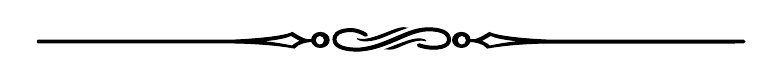
\begin{tikzpicture}
            \node (C) at (0,0) {};\node (D) at (9,0) {};
            \path (C) to [ornament=88] (D);
        \end{tikzpicture}
    \end{center}
\end{formal}

\subsection{其他符号}
这里给出其他的一些常用符号:

\begin{center}
\begin{tabular}{p{7em}p{12em}p{12em}}
    \toprule
    所需宏包 & 命令 & 效果 \\
    \hline
    none & \verb |\copyright| & \copyright \\
    none & \verb |\dag| & \dag \\
    none & \verb |\P| & \P \\
    none & \verb |\varpi| & $\varpi$ \\
    none & \verb |\bullet| & $\bullet$\\
    none & \verb |\clubsuit| & $\clubsuit$\\
    wasysym & \verb |\RHD| & $\RHD$ \\
    wasysym & \verb |\smiley| & \smiley\\
    marvosym & \verb |\Biohazard| & \Biohazard \\
    marvosym & \verb |\CEsign| & \CEsign\\ 
    marvosym & \verb |\Stopsign| & \Stopsign\\
    marvosym & \verb |\Radioactivity| & \Radioactivity \\
    marvosym & \verb |\Pointinghand| & \Pointinghand \\
    marvosym & \verb |\Writinghand| & \Writinghand \\
    pifont & \verb |\ding{227}| & \ding{227}\\
    dingbat & \verb |\smallpencil| & \smallpencil\\
    dingbat & \verb |\ding{229}| & \ding{229} \\
    manfnt & \verb |\lhdbend| & \scale{0.8}{\lhdbend}(缩放0.8)\\
    \bottomrule
\end{tabular} 
\end{center}


\section{首字下沉}
\begin{formal}{blue}
    \lettrine{S}{ome} textFirst-time space 
explorers welcome.Our universe is a wild and wonderful place. 
Join NASA astronauts, scientists, and engineers 
on a new adventure each week — all you need 
is your curiosity.
\end{formal}

\section{各个长度单位}
在 \LaTeX 中有着各种各样的单位,下面对这些单位进行可视化记忆:
\begin{example}
\begin{tabular}{l|l}
    \hline\\
    1.pt(point) & \red{\rule{1pt}{1pt}}\\
    \hline\\
    2.mm(毫米) &\red{\rule{1mm}{1mm}}\\
    \hline\\
    3.ex(size of 'x') &\red{\rule{1ex}{1ex}}\\
    \hline\\
    4.em(size of `M') &\red{\rule{1em}{1em}}\\
    \hline\\
    5.cm(厘米) &\red{\rule{1cm}{1cm}}\\
    \hline
\end{tabular}
\end{example}

\clearpage

\section{代码环境}
之前一直使用的是一个在线的网站,把导出的pdf插入tex文档,但是太麻烦了。
我之前也用过lslistings环境来定制我的代码抄录环境,但是效果还是不太理想,终于,
使用mint宏包可以较为满意。下面是两段插入代码示例:

\subsection{Cpp 代码}
\begin{code}{cpp}
int main()
{
    int i = 0;
    int j = 0;
    int N = 0;
    scanf("%d", &N);
    int ls[10] = {1, 2, 3, 4, 5, 6, 7, 8, 9, 10};
    for(i=0; i<N; i++){
        scanf("%d", &ls[i]);
    }
    return 0;
}
\end{code}

\subsection{Python 代码}
\begin{code}{python}
def add(x, y)
    return x+y
x = 1
y = 2
res = add(x, y)
\end{code}
\newpage



\section{自定义命令的坑}
我定义了一个常用的生成函数序列(\im{\fn{x}})的宏:
\begin{align}
    \fn{x}\\
    \fn[i]{x}
\end{align}

错误的调用例子:\verb |\fn[i]{x}| \par 
{
    \notice{注:调用LaTeX中自定义命令时:默认参数是放在[]内部的,不是\{\}内部}\par    
}


\noindent\textbf{颜色演示}【\small\texttt{注意:染色用textcolr,别用color(会影响你之后的所有内容)}】\par 
\fbox{
命令:\texttt{\textbackslash textcolor\{red\}\{hello 你好\}}, 结果: \textcolor{red}{hello 你好}}\\
\textbf{默认参数演示}\\
    \fbox{
        \parbox[t][7.5em]{0.45\linewidth}{
        错误命令:\\ \Cmd[\{第一个参数\}\{第二个参数\}]{Test} \\
        结果:\\ \Test{第一个参数}{第二个参数}   
    }}
    \hfill
    \fbox{
        \parbox[t][7.5em]{0.45\linewidth}{
        正确命令:\\ \texttt{\textbackslash Test[第一个参数]\{第二个参数\}} \\
        结果:\\ \Test[第一个参数]{第二个参数}
    }}

\section{公式相关}
\begin{itemize}
    \item 0. 普通形式:$\int_{i}^{\infty}$样例
    \item 1. \Cmd{displaystyle}形式(行间公式尺寸)
    \begin{itemize}
        \item 1.1 一个:$\displaystyle \int_{i}^{\infty}$样例
        \item 1.2 命令封装\im{\int_{i=0}^{\infty}{f(x,y) \Delta \xi_i}}
    \end{itemize} 
    \item 2. text形式(行内公式尺寸):$\textstyle{\int_{i}^{\infty}}$样例
    \item 3. scriptstyle形式(上下标尺寸): $\scriptstyle \int_{i}^{\infty}$
    \item 4. scriptscriptstyle(次级上下标尺寸): $\scriptscriptstyle \int_{i}^{\infty}$
    \item 5. Large参数尝试: \large{你好}
\end{itemize}


\subsection{上色}
\noindent\textbf{1.1  文本本生上色}\par 
\textcolor{red}{红色的文字}

\noindent\textbf{1.2 文本背景上色}\par 
\bbt{blue!20}{浅蓝色背景的字}

\noindent\textbf{2.1 公式本身上色}\par
\begin{equation}
    \color{blue!40}{\int_{i=0}^{\infty}{\sum_{i=0}^{\infty}{f(\xi_i,\varepsilon_i)} dx}}
\end{equation}

\noindent\textbf{2.2 公式背景上色}\par
\begin{align}
    \tcbhighmath{X_{k}} = 
    \tcbhighmath[colback=pink]{\frac{1}{N}\sum_{n=1}^{N-1}x_{n}e^{\mathrm{i}2\pi k\frac{n}{N}}}\\
    \bbf{blue!30}{\sum_{i=0}^{\infty}}
    \label{Test}
\end{align}

\subsection*{上色命令的封装}

\bbt{green!60}{浅绿色背景的文字}

\bbf{blue!30}{\sum_{i=0}^{\infty}}


\subsection{强制上下标}
\vspace*{2em}
\centerline{
    \shadowbox{强制下上标: $\sum\limits_{i=0}^{\infty}{\frac{1}{i^2}}$}    
}
但是\Cmd[]{limits}只能够应用于Operater(操作符).
比如 $\bowtie$ 就不是操作符,使用\Cmd[]{limits}强制下标就会报错.
此时可以使用\Cmd{mathop}把它转化成一个操作符,
然后就可以使用\Cmd[]{limits}了.\par 
使用演示:\par 
\begin{align}
    \mathop{\bowtie}\limits_{A\theta B}^{\sum\limits_{i=0}^{+\infty}{\displaystyle \int_{j=0}^{\mathop{\infty}\limits_{\scriptscriptstyle \sum_{\text{下标}}}^{\text{上标}}}{\frac{\mathop{1}\limits_{\text{Emoji}}^{\displaystyle \left.\cfrac{x}{2}\right|_{-\infty}^{+\infty}}}{i\cdot j\cdot x} {}d\left\{\mathop{x}\limits_{\iint}^{\displaystyle \oint_\Omega}\right\}}}}
\end{align}

\subsection{常见的limits变种}

\textcolor{blue!50}{注:以下的展示均为行内公式}

第一种,limits选项: \ensuremath{\int\limits_{a}^{b}{f(x) dx} }\hspace*{3em}\ensuremath{\sum\limits_{i=1}^{+\infty}}

第二种,nolimits选项: \ensuremath{\int\nolimits_{a}^{b}{f(x) dx} }\hspace*{3em}\ensuremath{\sum\nolimits_{i=1}^{+\infty}}

第三种:displaylimits: \ensuremath{\int\displaylimits_{a}^{b}{f(x) dx}} \hspace*{3em}\ensuremath{\sum\displaylimits_{i=1}^{+\infty}}


\subsection{加边框}
直接使用shadowbox就行了,如果最求简单一点的盒子,可以直接使用 boxed 命令,此命令内部会自动进入数学环境:

\shadowbox{$\sum_{i=1}^{+\infty}{\frac{1}{i^2}}=\frac{\pi^2}{6}$} \hfill
\boxed{\sum_{i=1}^{+\infty}{\frac{1}{i^2}}=\frac{\pi^2}{6}}


\subsection{\textbackslash \texttt{ensuremath}\{\}命令}
先看两个例子:\\
\fbox{
\parbox[t][3em][l]{0.4\linewidth}{
    命令:\texttt{\textbackslash ensuremath \{hello 你好\}}\\
    结果:\ensuremath{Hello 你好}
}}\hfill
\fbox{
\parbox[t][3em][l]{0.4\linewidth}{
    命令:\texttt{\{hello 你好\}}\\
    结果:Hello 你好
}}

\vspace*{2em}
由此可以看出\Cmd{ensuremath}会自动进入数学环境,这一点在自定义命令和环境时是十分有用的。
因为在 \verb |align| 等常见环境中可以嵌套此环境,但是你自定义命令中的含有 \verb |$ ** $|等,嵌入前面的环境
就会报错。



\section{TiKZ和GNUPlot结合}
在介绍怎么使用 TikZ 与 Gnuplot 之前,我们先说怎么编译。
在 \TeX 发行里,Gnuplot 并不包含在内。它的原理是 TikZ 调用
Gnuplot 之后,在编译的过程中,我们将会得到两个中间文件
\begin{itemize}
    \item 1. filename.pgf-plot.gnuplot
    \item 2. filename.pgf-plot.table
\end{itemize}
其中,前者是 pgf-plot.table 的设定文件,而后者就是调用 Gnuplot 
之后产生的一个数据表(点的坐标),然后 TikZ 调用这些点的坐标得到函数图。

为了能够使用 TikZ 与 Gnuplot,需要做两件事
\begin{itemize}
    \item 1. 在电脑安装 Gnuplot
    \item 2. 命令行:\texttt{pdflatex --shell-escape filename.tex},并且在vscode的配置文件中加上--shell-escape.
\end{itemize}
\begin{figure}[!htb]
    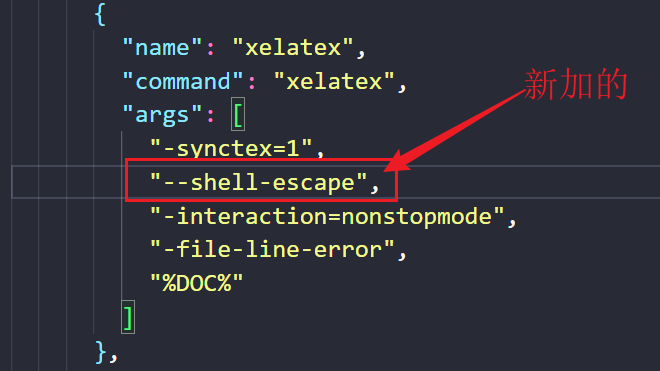
\includegraphics[scale=1]{JSON.png}
    \caption{VScode 配置GNU Plot}
\end{figure}
\newpage

\begin{formal}{blue}
代码
\begin{verbatim}
\begin{tikzpicture}[>=stealth]
    \tkzInit[xmin=-20,xmax=30,
                ymin=-350,ymax=50,
                xstep=10,ystep=100]
    \tkzAxeXY
    \tkzFct[domain=-12:26,color=magenta,thick]{14*\x-\x**2}
\end{tikzpicture}    
\end{verbatim}

\noindent 运行结果:
\begin{center}
    \begin{tikzpicture}[>=stealth]
        \tkzInit[xmin=-20,xmax=30,
                 ymin=-350,ymax=50,
                 xstep=10,ystep=100]
        \tkzAxeXY
        \tkzFct[domain=-12:26,color=magenta,thick]{14*\x-\x**2}
    \end{tikzpicture}
\end{center} 
这个例子用到了 tikz-fct 这个宏包,这个宏包的缺陷:
\begin{itemize}
    \item 1. 只有法文的手册,没法进行进一步的修饰。
    \item 2. 会出现字体的缺少警告.
\end{itemize}
\end{formal}

\newpage
\begin{formal}{red}
    由于上面的宏包没有英文版的手册,我们也只能看看别人的例子,
    下面给出 Gnuplot + pgfplots 结合的方法:
代码
\begin{verbatim}
\begin{tikzpicture}
\begin{axis}[axis x line = middle,
            axis y line = middle,
            xmin=-20,xmax=30,
            ymin=-350,ymax=70]
\addplot[domain=-12:26,color=orange,very thick,smooth] 
                            gnuplot {14*x-x^2};
\end{axis}
\end{tikzpicture}     
\end{verbatim}

\noindent 运行结果:
\begin{center}
\begin{tikzpicture}
    \begin{axis}[axis x line = middle,
                axis y line = middle,
                xmin=-20,xmax=30,
                ymin=-350,ymax=70]
    \addplot[domain=-12:26,color=orange,very thick,smooth] gnuplot {14*x-x^2};
    \end{axis}
\end{tikzpicture}        
\end{center}

% 不能够引入gnuplot的3d绘图功能
% \begin{center}
% \begin{tikzpicture}
%     \begin{axis}[axis x line = middle,
%                 axis y line = middle,
%                 xmin=-20,xmax=30,
%                 ymin=-350,ymax=70]
%     \addplot[] gnuplot {set isosamples 20,20; splot x**2+y**2 lt 7};
%     \end{axis}
% \end{tikzpicture}        
% \end{center}
\end{formal}     

\begin{mycolorbox}[red]{Remarque}
Our universe is a wild and wonderful place. 
Join NASA astronauts, scientists, and engineers 
on a new adventure each week — all you need 
is your curiosity. Visit the Amazon rainforest,
explore faraway galaxies and dive into our 
astronaut training pool. First-time space 
explorers welcome.
\end{mycolorbox}



\newpage
\section{页面布局相关设置}

\subsection{打印页面布局}
我们可以使用\texttt{layouts}宏包的 \texttt{layout}和\texttt{layout*} 命令可视化当前的页面布局

\bigskip
\begin{center}
\layout
\end{center}
\newpage

\subsection{图片任意放置}

我们可以使用\texttt{tikzpicture} 环境来进行图片的放置,本质上就是把node中的内容换位一张图片,
然后在这个环境上添加一个\texttt{overlay}参数,基本参数的作用解释:
\begin{itemize}
    \item \texttt{north west}: 页面的左上角
    \item \texttt{anchor}: 指定参考点来进行偏移
    \item \texttt{at}: 没有偏移时的位置
\end{itemize}

\begin{tikzpicture}[overlay, remember picture]
    \node[anchor=north east, xshift=0cm, yshift=0cm]
                        at (current page.north east)
    {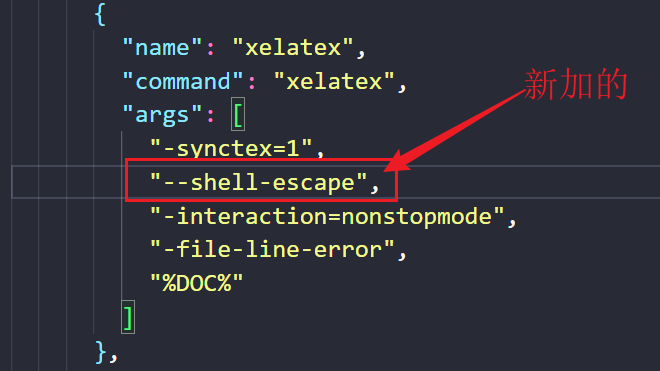
\includegraphics[width=3.3cm]{JSON.png}};
\end{tikzpicture}


%% 测试自定义的命令: 指定参考点, x位移, y位移【锚点方向为正】

\Rfig[south east]{JSON.png}{-15cm}{18cm}

\Rfig[south east]{JSON.png}{0cm}{8cm}

\Rfig[south west]{JSON.png}{0cm}{0cm};


\newpage
\subsection{图片文字环绕}
输出段落间距: \verb |\parindent |

% \setlength{\parindent}{0pt}
\begin{wrapfigure}[11]{r}{0.4\textwidth}
    \centering
    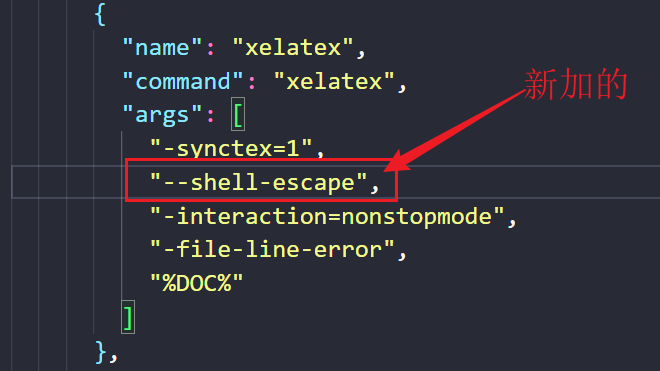
\includegraphics[scale=0.3]{JSON.png}
    \caption{FIG 1}
\end{wrapfigure}
\blindtext

%% 使用分段来解决图片到处跑的情况
%% 然后是的段间距=0pt即可
\begin{wrapfigure}[11]{l}{0.4\textwidth}
    \centering
    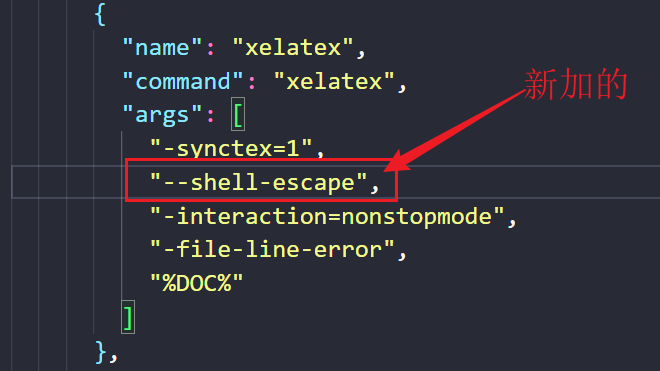
\includegraphics[scale=0.3]{JSON.png}
    \caption{FIG 2}
\end{wrapfigure}
\blindtext

\newpage
\subsection{单双栏排版}
\cmdindex{onecolumn,twocolumn}
\LaTeX{} 支持简单的单栏或双栏排版。标准文档类的全局选项 \texttt{onecolumn}、\texttt{twocolumn}
可控制全文分单栏或双栏排版。\LaTeX{} 也提供了切换单/双栏排版的命令:
\begin{command}
\cmd{onecolumn} \\
\cmd{twocolumn}\oarg{one-column top material}
\end{command}

\cmd{twocolumn} 支持带一个可选参数,用于排版双栏之上的一部分单栏内容。

\cmdindex{newpage,clearpage}
切换单/双栏排版时总是会另起一页(\cmd{clearpage})。
在双栏模式下使用 \cmd{newpage} 会换栏而不是换页;\cmd{clearpage} 则能够换页。

\cmdindex{columnwidth,columnsep,columnseprule}
双栏排版时每一栏的宽度为 \cmd{columnwidth},它由 \cmd{textwidth} 减去 \cmd{columnsep} 的差除以 2 得到。
两栏之间还有一道竖线,宽度为 \cmd{columnseprule},默认为零,也就是看不到竖线。

\cmdindex{columnwidth,columnsep,columnseprule}
双栏排版时每一栏的宽度为 \cmd{columnwidth},它由 \cmd{textwidth} 减去 \cmd{columnsep} 的差除以 2 得到。
两栏之间还有一道竖线,宽度为 \cmd{columnseprule},默认为零,也就是看不到竖线。

\pkgindex{multicol}
\envindex[multicol]{multicols}
一个比较好用的分栏解决方案是 \pkg{multicol},它提供了简单的 \env{multicols} 环境
(注意不要写成 \env{multicol} 环境)自动产生分栏,如以下环境将内容分为 3 栏:
\begin{verbatim}
\begin{multicols}{3}
...
\end{multicols}
\end{verbatim}


\subsubsection{使用\textbackslash twocolumn命令}
\red{缺点:无法在一页中使用单栏,双栏并存。使用$\backslash$newpage进行换列}
\twocolumn
\columnseprule=0.5pt
双腿瘫痪后,我的脾气变得暴怒无常。望着望着天上北归的雁阵,我会突然把面前的玻璃砸碎;听着听着李谷一甜美的歌声,
我会猛地把手边的东西摔向四周的墙壁。母亲就悄悄地躲出去,在我看不见的地方偷偷地听着我的动静。当一切恢复沉寂,
她又悄悄地进来,眼边红红的,看着我。“听说北海的花儿都开了,我推着你去走走。”她总是这么说。母亲喜欢花,可自从我的腿瘫痪后,
她侍弄的那些花都死了。“不,我不去!”我狠命地捶打这两条可恨的腿,喊着:“我活着有什么劲!”母亲扑过来抓住我的手,
忍住哭声说:“咱娘儿俩在一块儿,好好儿活,好好儿活……”可我却一直都不知道,她的病已经到了那步田地。后来妹妹告诉我,
她常常肝疼得整宿整宿翻来覆去地睡不了觉。

那天我又独自坐在屋里,看着窗外的树叶“唰唰拉拉”地飘落。母亲进来了,挡在窗前:“北海的菊花开了,我推着你去看看吧。
”她憔悴的脸上现出央求般的神色。“什么时候?”“你要是愿意,就明天。”她说。我的回答已经让她喜出望外了。“好吧,就明天。”我说。
她高兴得一会坐下,一会站起:“那就赶紧准备准备。”“唉呀,烦不烦?几步路,有什么好准备的!”她也笑了,坐在我身边,
絮絮叨叨地说着:“看完菊花,咱们就去‘仿膳’,你小时候最爱吃那儿的豌豆黄儿。还记得那回我带你去北海吗?你偏说那杨树花是毛毛虫,
跑着,一脚踩扁一个……”她忽然不说了。对于“跑”和“踩”一类的字眼儿。她比我还敏感。她又悄悄地出去了。
\newpage 
%% 注意:此处的换页是换栏
%% 换页使用\clearpage
她出去了。就再也没回来。

邻居们把她抬上车时,她还在大口大口地吐着鲜血。我没想到她已经病成那样。看着三轮车远去,也绝没有想到那竟是永远的诀别。

邻居的小伙子背着我去看她的时候,她正艰难地呼吸着,像她那一生艰难的生活。别人告诉我,她昏迷前的最后一句话是:“我那个有病的儿子和我那个还未成年的女儿……”

又是秋天,妹妹推我去北海看了菊花。黄色的花淡雅、白色的花高洁、紫红色的花热烈而深沉,泼泼洒洒,秋风中正开得烂漫。我懂得母亲没有说完的话。妹妹也懂。我俩在一块儿,要好好儿活……
\clearpage
\onecolumn
% \clearpage
\red{\textbf{赏析}}\par
{
    \kaishu
    世界上最痛苦的事情莫过于“子欲养而亲不待”,这样的痛楚太过绵长,痛得难以名状。

    随着年龄的增长,时间长河的流逝,我们会慢慢离开父母温馨的怀抱。为学习,为工作,为生活,和父母甚至远隔万水千山。
    一家人在一起的日子终究是有限的,珍惜和父母在一起的日子。在面临突如其来的困难时,不要太过任性,不要自暴自弃,
    要知道如果你觉得痛苦了,父母所承受的痛苦是加倍的,爱自己,“好好活”,也是爱父母。

    作者寥寥几百字就把自己对母亲的爱与自己少不更事的追悔挥洒得淋漓尽致,表现了母爱的无私、理解与伟大。
}
\newpage

\subsubsection{使用multicolomn宏包}

% \usepackage{multicol}

{
    \red{
    \begin{itemize}
        \item 1. 在multipulcols*环境中 --> 默认一个分栏排满以后在换栏。
        \item 2. 在multicols(*)环境中使用$\backslash$newpage只会换到新的一页
        \item 3. 使用$\backslash$columnbreak来换栏
    \end{itemize} 
    }   
}
\par
\vspace*{4em}
\centerline{\red{\textbf{伟大与渺小- -臧克家}}}
\begin{multicols}{2}

我们有太多的伟人。写在历史上的被渲染过的,不必说他们了;和我们同时代,向我们显示伟大的,已经够数了。
这些人,凭了个人的阴谋机诈、凭了阴险与残酷,只要抓住一个机会使自己向高处爬一级,他是决不放弃这个机会的,
至于牺牲个人的天良与别人的利害甚至生命,他毫不顾惜。这些伟人的伟大,是用个人的人性去换来的,是踏在人民大众的骨骸上升高起来的。
当他站得高、显得伟大的时候,一般有肉没有骨头,有躯壳没灵魂的人中狗,便成群地蜷伏在他脚下,仰起头来望望他,便“伟大呵,
伟大呵”地乱叫一阵子。当别人靠近他的时候,它们便狺狺狂吠起来,在壮主子的声威之余,自己仿佛也有威可畏了。这些伟人与臣侯是相依为命,
狼狈为奸的。主子为了获取权势的兔,是不能没有走狗的,在走狗的瞳孔里,主子的尊容也许并非那样庄严,然而在他们口里又是另一回事了。
为了一块骨头,它们出卖了自己。
% \columnbreak
在伟人自己,眼睛看的是逢迎的脸色,咂嚅趑趄的情感,耳朵听的是谗媚阿佞的声音,左右的人钢壁铁墙一样把他围在一个小天地里,眼看不过咫尺,
耳听不出左右,久而久之,也只能以他人之耳为耳,以他人之目为目。
% \newpage
\columnbreak

而这些他人,又正是以他为法宝而有所贪图的人,他们所说的话,所报告的见闻,
全是以自己的利害为标准而取舍,改窜,编辑的,不但与事实不符,常常会整个相反。

信假为真,以真为假,是非颠倒,黑白不分。
古时候有这样的皇帝,天下大饥,他怪罪人民何不食肉糜,今日的伟人吃的鸡蛋也许还是一块钱一个。

这样的伟人,拔地几千尺,活在半空里,和群众、和现实,脱离得一干二净。在别人眼前,他作势,他装腔,他在别人眼里不是“人”,而是“伟人”。
他自己,喜怒哀乐,不能自由,不愿自由,不敢自由,硬把人之所以为人的一些天性压抑,闷死,另换上一些人造的东西,这样弄得长久了,
自己也觉得自己不是“人”了,而成了“人”以上的另一种人的“人”。勉强解释,就是孤家“寡人”之“人”。这样的“人”,是“性相近也,习相远也”,
远的是民众,是人性。这样的人是刚愎的,残暴的,虚伪的,反动的,半疯狂的,自欺欺人的,存心“不令天下人负我,我负天下人”的。
把一个国家,一个世界,交给这样一个半疯子去统治,那会造成个什么样子呢?

\end{multicols}
\red{\textbf{赏析}}\par
{
    \kaishu 
    苍茫大地,芸芸众生中,每个人都是渺小的,不需要因为自己的渺小而感到自卑,渺小有渺小的妙处,每个人都有自己的位置,
    都能找到自己的光源,发出自己的声音。要知道蓝天有自己的深邃,白云有自己的飘逸,草原有自己的芬芳,
    就连不起眼的小草也有属于自己的翠绿,每个人都是独特而优秀的
}

\subsection{浮动体}
内容丰富的文章或者书籍往往包含许多图片和表格等内容。这些内容的尺寸往往太大,导致
分页困难。\LaTeX 为此引入了浮动体的机制,\red{令大块的内容可以脱离上下文,放置在合适的位置}。
LATEX 预定义了两类浮动体环境 figure 和 table。习惯上 figure 里放图片,table 里放
表格,但并没有严格限制,可以在任何一个浮动体里放置文字、公式、表格、图片等等任意内容。


\textbf{各个参数的理解}\par
\Arg{placement} 参数提供了一些符号用来表示浮动体允许排版的位置,\red{如 \texttt{hbp} 允许浮动体排版在当前位置、底部或者单独成页}。
\env{table} 和 \env{figure} 浮动体的默认设置为 \texttt{tbp}。
\begin{table}[htp]
\centering
\caption{浮动体的位置参数}\label{tbl:float-placement}
\begin{tabular}{*{2}{l}}
 \hline
 \textbf{参数} & \textbf{含义} \\
 \hline
 \texttt{h} & 当前位置(代码所处的上下文) \\
 \texttt{t} & 顶部 \\
 \texttt{b} & 底部 \\
 \texttt{p} & 单独成页 \\
 \texttt{!} & 在决定位置时忽视\red{限制} \\
 \hline
\end{tabular}
\begin{quote}\footnotesize
注 1:排版位置的选取与参数里符号的顺序无关,\LaTeX{} 总是以 \texttt{h-t-b-p} 的优先级顺序决定浮动体位置。
也就是说 \texttt{[!htp]} 和 \texttt{[ph!t]} 没有区别。\par
注 2:限制包括\red{浮动体个数}(除单独成页外,默认每页不超过 3 个浮动体,其中顶部不超过 2 个,底部不超过 1 个)
以及\red{浮动体空间占页面的百分比}(默认顶部不超过 70\%,底部不超过 30\%)。
\end{quote}
\end{table}

\section{盒子}
一般的水平盒子,竖直盒子在 lshort 上面都讲地清清楚楚的,具体参见lshort。
盒子是 \LaTeX 排版的基础单元,虽然解释上去有些抽象:每一行是一个盒子,里面的文字从
左到右依次排列;每一页也是一个盒子,各行文字从上到下依次排布,颇有一些活字印刷术的
味道。\par
不管如何,\LaTeX 提供了一些命令让我们生成一些有特定用途的盒子。
\subsection{水平盒子}
\begin{command}
    \cmd{mbox}\marg*{\ldots} \\
    \cmd{makebox}\oarg{width}\oarg{align}\marg*{\ldots}
\end{command}
\cmd{mbox} 生成一个基本的水平盒子,内容只有一行,不允许分段(除非嵌套其它盒子,比如后
文的垂直盒子)。外表看上去,\cmd{mbox} 的内容与正常的文本无二,不过断行时文字不会从盒子里
断开。

\textbf{测试}\par
\mbox{生成一个基本的水平盒子,内容只有一行,不允许分段(除非嵌套其它盒子,比如后
文的垂直盒子)。\\外表看上去,\cmd{mbox} 的内容与正常的文本无二,不过断行时文字不会从盒子里
断开。
}

{
    \kaishu
    \textsf{结论:}
    从上便可以看出, $\backslash \backslash$不起作用, 也不会自动换行
}

\subsection{自定义水平盒子}
对齐选项有:
\begin{itemize}
    \item c:居中对齐(默认)
    \item l:左对齐
    \item r:右对齐
    \item s:分散对齐
\end{itemize}
\textbf{测试}\par

\begin{enumerate}
    %% \boxed 可以显示盒子的形状
    %% 换行符\\会在下一行产生一个盒子
    \item \fbox{\mbox{Test 10em box}}
    \item \fbox{\makebox[10em][c]{Test 10em box}}\\
    \item \fbox{\makebox[10em][s]{Test 10em box}}\footnote[1]
    {分散对齐方式强行拉开单词的间距,
    往往会报 Underfull $\backslash$hbox 的消息}
\end{enumerate}    


\textbf{水平盒子加边框}

\begin{command}
    \cmd{fbox}\marg*{\ldots} \\
    \cmd{framebox}\oarg{width}\oarg{align}\marg*{\ldots}\\
    \cmd{boxed}\marg*{\ldots}
    通过 \cmd{setlength} 命令调节边框的宽度(向外拓展) \cmd{fboxrule} 和内边距(保证上下内边距) \cmd{fboxsep} 
\end{command}


\begin{example}
    %% 1.\boxed{}会自动进入数学环境
    %% \boxed{} 和 \fbox{} 不能指定宽度和对齐
    %% 2. ~会输出硬空格
    \boxed[10em]{Hello~}\\
    \boxed{Hello~}\\
    \boxed{\sum_{i=0}^{\infty}{\frac{1}{i^2}}}\\
    \fbox{Hello Jack}\\
    \framebox[3em][l]{Helloa}\\
    \framebox[3em][l]{MMM}\\

    \framebox[6em][l]{Hello}

    \setlength{\fboxrule}{5mm}
    \framebox[6em][l]{Hello}\\

    \setlength{\fboxsep}{10mm}  
    \framebox[6em][l]{Hello}

\end{example}

\subsection{竖直盒子}
\textbf{一般是可以换行的}\par
\begin{command}
    \cmd{parbox}\oarg{align}\oarg{height}\oarg{inner-align}\marg{width}\marg*{\ldots} \\[0.5ex]
    \cmd{begin}\marg*{minipage}\oarg{align}\oarg{height}\oarg{inner-align}\marg{width} \\
    \ldots \\
    \cmd{end}\marg*{minipage}
\end{command}

\textbf{测试}\par
\begin{example}
测试:\parbox[b][2em][r]{3em}%
    {你好, what you do, Thanks}    
\end{example}


\vspace*{4em}
\begin{example}
测试:\parbox[b][2em][r]{3em}%
    {你好, what you do, Thanks}    
\end{example}

\vspace*{4em}
\begin{example}
测试:\parbox[t][2em][r]{4em}%
    {你好, what you do, Thanks}    
\end{example}


\vspace*{4em}
\begin{example}
测试:\parbox[t]{4em}%
    {你好, what you do, Thanks}    
\end{example}

\vspace*{4em}
\begin{example}
\fbox{  
    测试:\parbox[b][2em][c]{8em}%
    {你好, what you do, Thanks}  
    }  
\end{example}

\vspace*{4em}
\begin{example}
\textcolor{red}{测试}:\parbox[t]{8em}%
    {北美洲原始居民为印第安人。16-18世纪,
    正在进行资本原始积累的西欧各国相继入侵北美洲。
    到了十八世纪中期,在北美大西洋沿岸建立了
    十三块殖民地,殖民地的经济,文化,政治相对
    成熟。}  
\end{example}


\vspace*{4em}
\begin{example}
\textcolor{red}{测试}:\parbox[b]{8em}%
    {北美洲原始居民为印第安人。16-18世纪,
    正在进行资本原始积累的西欧各国相继入侵北美洲。
    到了十八世纪中期,在北美大西洋沿岸建立了
    十三块殖民地,殖民地的经济,文化,政治相对
    成熟。}  
\end{example}

{
    \kaishu 
    总结,一般使用格式\\
    1.\cmd{parbox} [\oarg{parbox盒子和前边盒子的对齐方式}]\{<text>\}\\
    2.\\
    \cmd{begin}\marg*{minipage}\par
    \oarg{minipage盒子和前边盒子的对齐方式}\par
    \oarg{\oarg{minipage盒子的高度}}\par
    \oarg{minipage盒子内部的对齐方式}\par
    \marg{\oarg{minipage盒子的宽度}}\par
    <text>\\
    \cmd{end}\marg*{minipage}
}

\subsection{标尺盒子}
\cmd{rule} 命令用来画一个实心的矩形盒子,也可适当调整以用来\textcolor{red}{画线}(标尺):
\begin{command}
\cmd{rule}\oarg{raise}\marg{width}\marg{height}
\end{command}
\begin{example}
Black \rule{12pt}{4pt} box.

Upper \rule[4pt]{6pt}{8pt} and
lower \rule[-4pt]{6pt}{8pt} box.

A \rule[-.4pt]{3em}{.4pt} line.
\end{example}

本质上也就是画一个粗的实心矩形,具体的使用样例如下:我绘制了一个宽\verb |0.8\linewidth|, 高5pt, 离开基线 0pt的一个居中矩形。


代码如下:
\begin{verbatim}
\begin{center}
    \textcolor{blue}{
        \rule[0pt]{0.8\linewidth}{5pt}
    }
\end{center}
\end{verbatim}

绘制效果:
\begin{center}
    \textcolor{blue}{
        \rule[0pt]{0.8\linewidth}{5pt}
    }
\end{center}


\subsection{缩放盒子}
我们可以使用缩放盒子完成一些很伟大的操作。还记得有一次我想用LaTeX的logo绘制一个封面,结果绘制出来的那个logo太小了,
只有放大AI里面操作一番之后再在插入进来,极尽狼狈。现在直接使用 LaTeX 的graphicx宏包使用的缩放功能就行了,可以实现对几乎任何的对象
进行缩放:图片,文字,数学符号, ...
自定义的源代码演示:
\begin{verbatim}
\newcommand{\scale}[3]{
    \scalebox{#1}[#1]{#2}
}
\end{verbatim}

具体的使用效果:放大了3倍的 TeX logo

\begin{center}
    \scale{3}{\TeX}\hspace*{0.4\linewidth} \scale{3}{$\sum$}
\end{center}

\subsection{旋转盒子}
这个{\ttfamily rotatebox}命令必须放在figure环境中,从下面也可以看出,box对象,旋转的基点是左下角,在基线上

%% 错误的命令
\begin{figure}[!htb]
    \begin{tikzpicture}[overlay, remember picture]
        % \node[] at (0, 0) {};
        \draw[ultra thick, red](0, 0)node[below] {\textcolor{red}{\kaishu 基线}}--(1\linewidth, 0);
    \end{tikzpicture}
    \rotatebox{45}{%
    \begin{minipage}[t]{0.3\linewidth}
        % 注意:如果不用centering的话, caption无法对齐
        \centering
        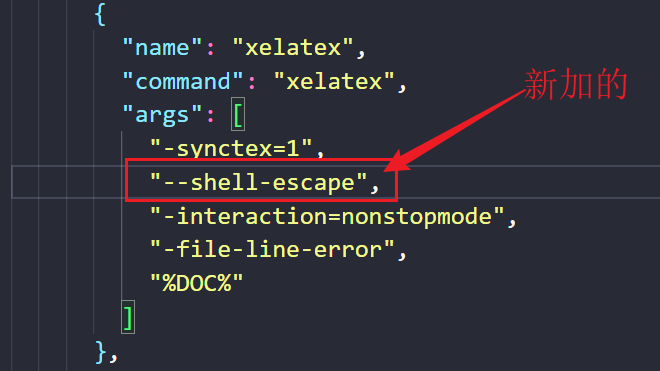
\includegraphics[scale=0.2]{JSON.png}
        \caption{逆时针45度} 
    \end{minipage}}
    \hfill
    \begin{minipage}[t]{0.3\linewidth}
        % 注意:如果不用centering的话, caption无法对齐
        \centering
        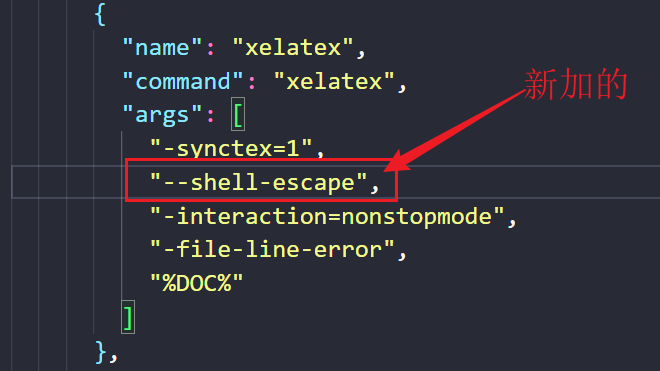
\includegraphics[scale=0.2]{JSON.png}
        \caption{没有旋转} 
    \end{minipage}
    \hfill
    \rotatebox{-45}{%
    \begin{minipage}[t]{0.3\linewidth}
        \centering
        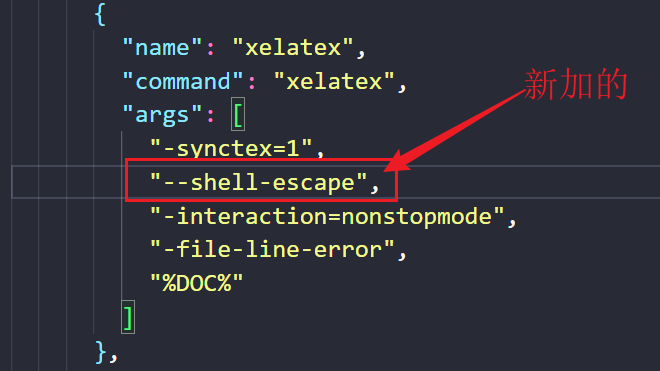
\includegraphics[scale=0.2]{JSON.png}
        \caption{顺时针45度} 
    \end{minipage}}
\end{figure}

\newpage


\section{一些primitive}
当我们想要魔改一些东西的时候,我们必须的使用内部的宏,这是不可避免的。下面介绍几个基本的原语(primitive):
我们通过一个例子来引入:

\subsection{\TeX 的背后}

\textbf{下面为一些尝试的命令}

命令一:\verb |T\kern-0.2em\lower.25em\hbox{E}\kern-0.1em X|

命令二:\verb |\ensuremath{\mathrm{L\kern-.325em{\scriptstyle{A}}\kern-.17em}}\TeX|

% 命令三:L\kern-.325em\hbox{\check@mathfonts\fontsize\sf@size\z@\math@fontsfalse\selectfont A}\kern-.17em\TeX

运行效果:T\kern-0.2em\lower.25em\hbox{E}\kern-0.1em X~~~~\ensuremath{\mathrm{L\kern-.325em{\scriptstyle{A}}\kern-.17em}}\TeX

正如上面的代码所示,主要就是一个lower宏,使用+,-可以实现上下偏移。例如,我们把lower后面的
正号变为 -时,E机会出现在上面, \LaTeX 中的A同理

效果演示一:T\kern-0.1em\lower-.25em\hbox{E}\kern-0.1em X 

效果演示二:L\kern-0.2em\lower0.3em\hbox{A}\kern-0.2emT\kern-0.1em\lower-.25em\hbox{E}\kern-0.1em X

\clearpage
\subsection{primitive介绍}
\begin{itemize}
    \item 1. \textbackslash kern:  其中 -  表示向左移动
    \item 2. \textbackslash lower: 其中 - 表示向上移动
    \item 3. \textbackslash raise: 其中 - 表示向下移动
    \item 4. \textbackslash hbox: 表示水平盒子
\end{itemize}

\begin{tformal}{\LaTeX 的原始命令}
\begin{verbatim}
\DeclareRobustCommand{\LaTeX}{L\kern-.36em%
    {\sbox\z@ T%
        \vbox to\ht\z@{\hbox{\check@mathfonts
                            \fontsize\sf@size\z@
                            \math@fontsfalse\selectfont
                            A}%
                    \vss}%
    }%
    \kern-.15em%
    \TeX}
\end{verbatim}
\end{tformal}

\section{魔改系列}
\subsection{进制}
在 \TeX 的内部使用  \verb |'(单引号)|后加数字表示八进制,\verb |"(双引号)|后接数字表示十六进制。
下面便有几个示例。注:我们使用原语(primitive)的\verb |\number|命令进行十进制输出.

\begin{figure}[!htb]
    \centering
    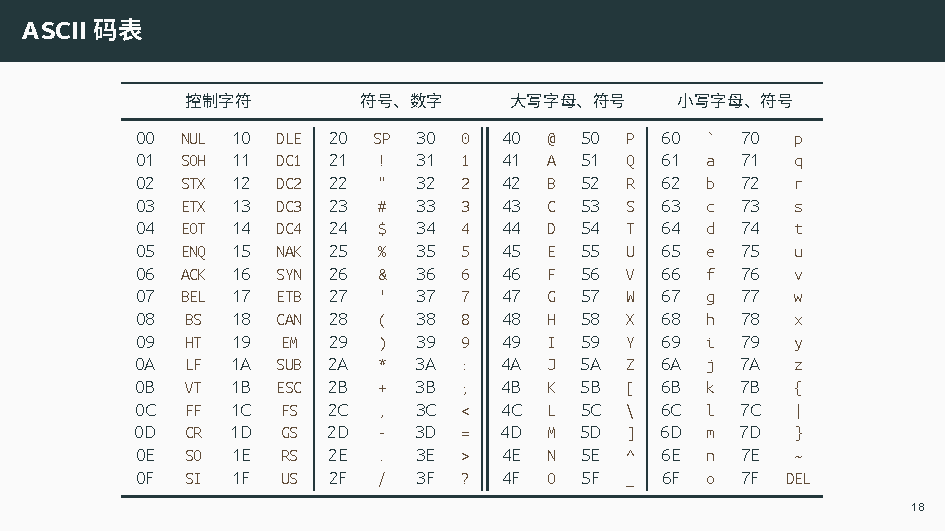
\includegraphics[scale=1]{ASCII.pdf}
    \caption{ASCII}
    \label{ASCII}
\end{figure}

八进制:\verb|\number'10| ~~~ 结果:\number'10

十进制:\verb|\number10| ~~~ 结果:\number10

十六进制:\verb|\number"10| ~~~ 结果:\number"10

\subsection{\TeX\ 的字符与编码}
\TeX\ 内部的字符是有各自的编码的,下面先演示一句话:

神秘代码:\verb |^^(^^%^^,^^,^^/^^l^^`^^7^^/^^2^^,^^$^^a|

运行结果:^^(^^%^^,^^,^^/^^l^^`^^7^^/^^2^^,^^$^^a

实际的对应规则:就是下面\ref{ASCII}那个 ASCII 码表左右两列对应字符的相互对应

具体的规则如下:

\begin{itemize}
    \item 1. 连续两个上标符号 \verb|^^| 后跟一个字符 c,可以表示另一个字符 \ensuremath{c'}
    \begin{itemize}
        \item 1.1 64 $\mathrm {\le ASCII_c \le 127 \Rightarrow ASCII_{c'} = ASCII_c - 64}$
        \item 1.2 0 $\mathrm {\le ASCII_c \le 63 \Rightarrow ASCII_{c'} = ASCII_c - 64}$
    \end{itemize}
    \item 2. \verb |^^| 后跟两个{\bf 小写}十六进制数字,可以表示任意 ASCII 符号
\end{itemize}

下面演示第二点:

代码:\verb |^^68^^65^^6c^^6c^^6f^^2c^^20^^77^^6f^^72^^6c^^64^^21|

运行结果:^^68^^65^^6c^^6c^^6f^^2c^^20^^77^^6f^^72^^6c^^64^^21

\subsection{字符\&编码的转换}
我们可以使用原语 \verb |\number| 轻松的输出字符对应的ASCII数值\footnote{注:ASCII中的字符和十进制之间的相互转换}
\begin{itemize}
    \item 1. 字符 $\Rightarrow$ 编码:\verb |`<字符>|
    \item 2. 编码 $\Rightarrow$ 字符:\verb |\char<编码>|
\end{itemize}

\begin{tcolorbox}[colback=red!5!white,colframe=red!75!black,title=注意]
 编码转换使用的是前引号: \verb |`|, 但是8进制使用的是后单引号: \verb |'| 
\end{tcolorbox}


下面展示关于字符到编码的几个使用样例:

代码:\verb |\number`A| ~运行结果:\number`A

代码:\verb |\number`\A| 运行结果:\number`\A

代码:\verb |\number"41| 运行结果:\number"41

代码:\verb |\number`\%| 运行结果:\number`\%


\noindent 但是如果我们输入了 \verb |\number `人|,即一个非ASCII字符\footnote{注意:pdflatex不支持Unicode编码}那么会得到什么东西呢?

代码:\verb |\number`人| 运行结果:\number`人

\noindent 其实此时它会按照Unicode字符集进行映射。

下面再展示几个编码到字符的转换样例:

代码:\verb |\char65| ~运行结果:\char65

代码:\verb |\char"41| ~运行结果:\char"41

代码:\verb |\char20000| ~运行结果:\char20000

我们可以使用 \verb |\char|命令进行一些不方便使用输入法键入的繁体字的录入,前提是我们得知道它的 Unicode 
编码\footnote{默认情况下xelatex使用的字体是latin morden,其中只有拉丁字母,不含中文}。
所以必要时你需要指定一个支持中文, 且支持中文数量比较的字体,使用如下的语句进行设置:

\begin{verbatim}
\usepackage{fontspec}
\setmainfont{SimSun}
\end{verbatim}


\subsection{类别码}
相关的注意事项,主要就是下面的两张表

\vspace*{6em}
\begin{figure}[!htb]
    \centering
    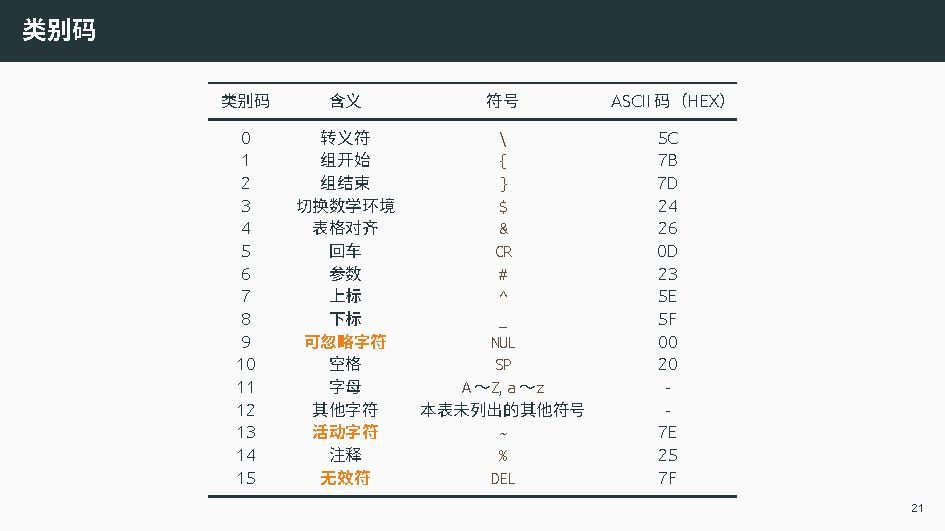
\includegraphics[scale=1]{catcode.pdf}
    \label{catcode}
    \caption{catcode}
\end{figure}

\begin{figure}[!htb]
    \centering
    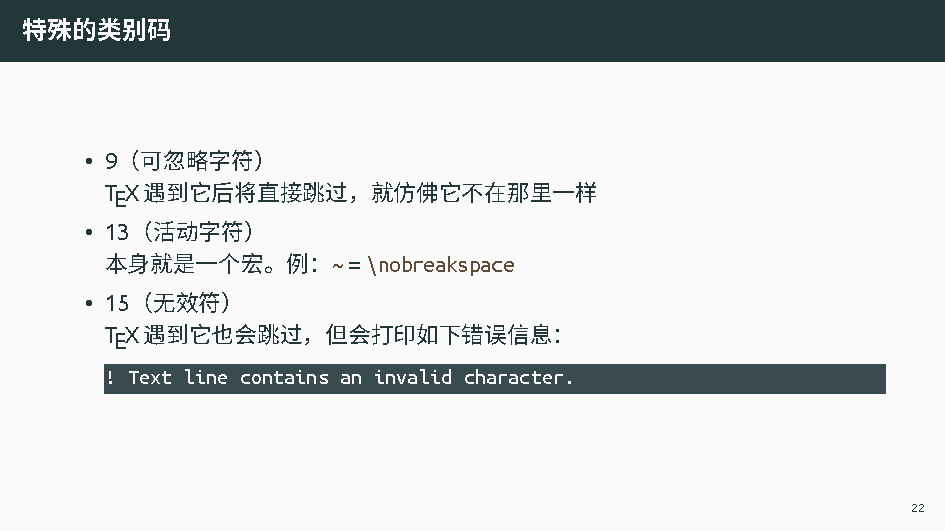
\includegraphics[scale=1]{catcode2.pdf}
    \caption{catcode2}
    \label{catcode2}
\end{figure}

\newpage

\subsection{@ 溯源} 

\begin{framed}
    \begin{minipage}[t]{0.45\linewidth}
        首先展示一段代码:
        \begin{verbatim}
    \makeatletter
    \number\@ne

    \number\thr@@
    \makeatother  
        \end{verbatim}
    \end{minipage}
    \hfill
    \begin{minipage}[t]{0.45\linewidth}
        它的运行结果如下:

        \makeatletter
        \number\@ne

        \number\thr@@
        \makeatother

        其实在 \LaTeX 2 $\varepsilon$ 中:

        \verb |\@ne = 1| \hspace*{3em} \verb |\tw@ = 2|

        \verb |\thr@@ = 3| \hspace*{3em} \verb |\sixt@@n = 16|

        还有其它的很风骚的命名,具体可以参见官方文档:macros2e
    \end{minipage}
\end{framed}


tex将字符分成16类(catcode),其中第11类是letter(a-z, A-Z),第12类是other,
就是除了其它15类的那种。tex命令只能由letter组成(这也是很多人在macro名中
用数字出错的原因,数字就属于other类)。@默认属于other类,故不能在macro的名字中出现。
LaTeX的内部命令中,\verb |\makeatletter| 命令的实质就是修改字符@的catcode为11,
这样@就可以出现在命令名称中了。\verb |\makeatother| 重新修改@的catcode为12,不允许@出现在命令的名字中。 


\newpage
\subsection{catcode 背锅}
catcode 就是 TeX 的一个黑魔法,当你学会了使用 catcode,并且随意使用这玩意之后,你的 LaTeX 代码就没有人能够看得懂了。

下面开始使用catcode命令魔改TeX:
\begin{figure}[!htb]
    \centering
    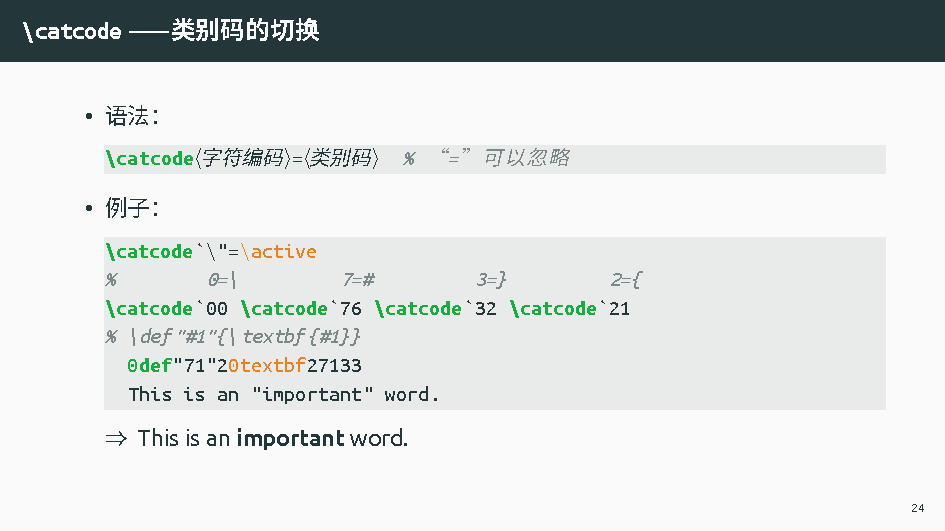
\includegraphics[scale=1]{catcode3.pdf}
    \caption{catcode3}
    \label{catcode3}
\end{figure}

\end{document}

